\subsubsection{Concept 1}

Shape memory alloys (SMAs) such as Nitinol may be useful for mimicking the grasping of a plant tendril. SMAs transition to
a superelastic state above a threshold temperature. In this state, they are rigid and retain their shape. Below the threshold
temperature, they are malleable. They have the unique property of returning to their "remembered" superelastic when heated back
above the threshold temperature. SMAs have a high strength to weight ratio and due to their malleability can be used for the design of
actuators that mimic organic shapes such as a spiraling plant tendril \cite{baek_dexterous_2023}.
The downside of SMAs in this application is that in order to hold their superelastic form, they must remain heated \cite{wieczorek_smart_2018}.
This would mean the drone must supply current to the grasper to maintain its temperature. This power consumption would negate many of the benefits
of perching, so a method for the grasper to passively hold its position would be needed.


The jamming transition could allow a tendril like actuator to passively hold its position by changing from a flexible form
to a rigid one. With jamming, a volume of particulate matter is held in a flexible container. It is free to be deformed by
external forces until a partial vacuum is applied, after which atmospheric pressure forces the particles to interlock and act
as a solid. This can be accomplished with overlapping sheets or fibers instead of particles as well \cite{fitzgerald_review_2020}.
An example of this is the Universal Gripper \cite{brown_universal_2010}, in which a balloon filled with coffee grounds can
be used to grasp a wide variety of objects. First the balloon is pressed against the object to form to its shape, then a vacuum is
applied and the balloon assumes a rigid form around the object.  


This concept consists of an actuator with 3 SMA wires and a granular core (see Fig. {fig:poses}) cabable 
of transitioning between a flexible and stiff phase via the jamming transition. Jamming will be achieved by 
a syringe-like pump that can draw air out of the core.

The actuator will use SMA wires to actively transition between 3 positions shown in Fig. {fig:poses}:
\begin{itemize}
    \item Home: the tendril is tightly coiled near the drone so as to not obstruct flight.
    \item Extended: The tendril is extended straight up from the drone, for positioning adjacent to a perch.
    \item Coiled: The tendril coils so as to grasp a nearby branch within it.
\end{itemize}
Each transition will be driven by one SMA wire, each wire will be actuated through Joule heating that is activated by the flight controller.



\begin{figure}[H]
    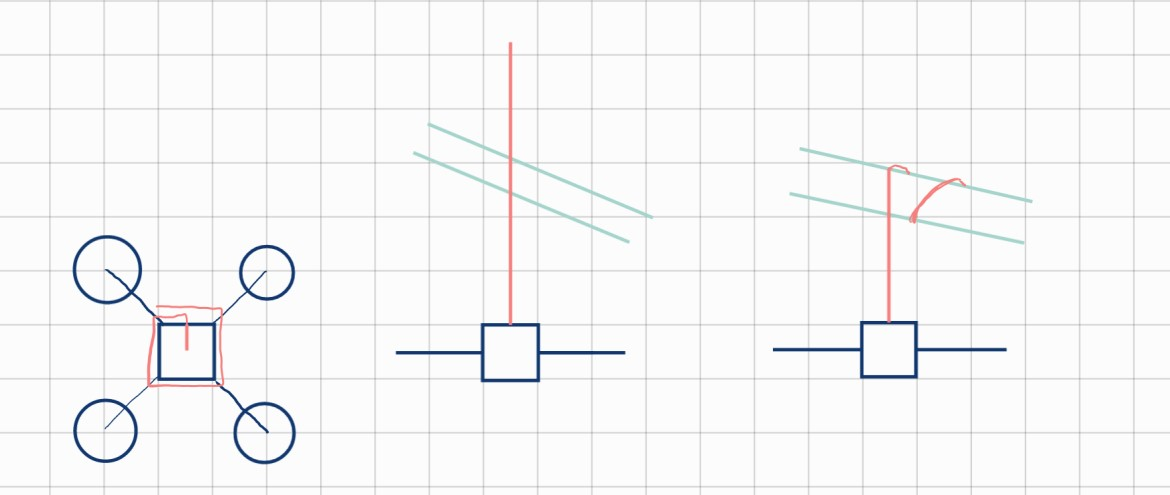
\includegraphics[width=\textwidth]{Poses.jpg}
    \caption{The 3 poses that the actuator (red) will achieve. Home position (left) has the grasper coiled near the drones
    body (blue), for unencumbered flight. In extended position (center) the device reaches straight above the drone to be
    positioned adjacent to a perch (green). While coiled (right), the end of the device grasps around the perch, with some
    length uncoiled so that the drone hangs below the perch.}
    \label{fig:poses}
\end{figure}


A core designed to transition between flexible and solid via the jamming transition (Fig. {fig:crosssec}) will allow the tendril to remain
securely attached when power is removed from the SMA wires. This may be a tube filled with coffee grounds or similar
particles, or it may utilize friction between layers of other material.


\begin{figure}[H]
    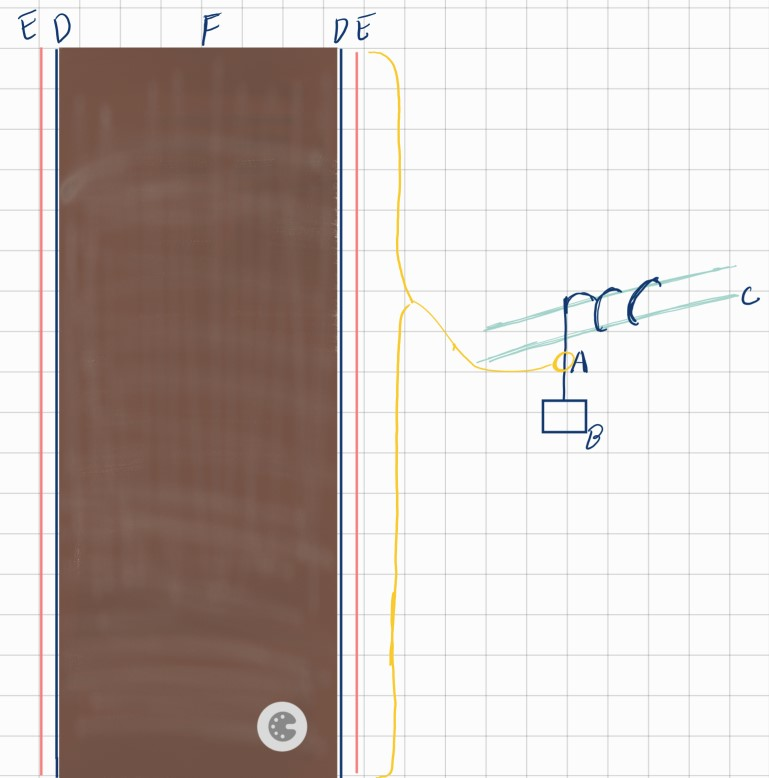
\includegraphics[width=\textwidth]{diagram.jpg}
    \caption{Sketch of the proposed device. The right side shows the device (A)
    attaching a drone (B) to a perch (C). The view on the left shows the flexible core of the device (D),
    two of the 3 SMA wires intended to transition between two positions (E) and the particulate core facilitating
    jamming (F). }
    \label{fig:crosssec}
\end{figure}


The jamming transition will be controlled by a syringe-like linear pump, driven by a servo that is also controlled by the drones flight controller.
Fig. {fig:schematic} shows a simple diagram of the electrical and mechanical components involved in the proposed device.  


\begin{figure}[H]
    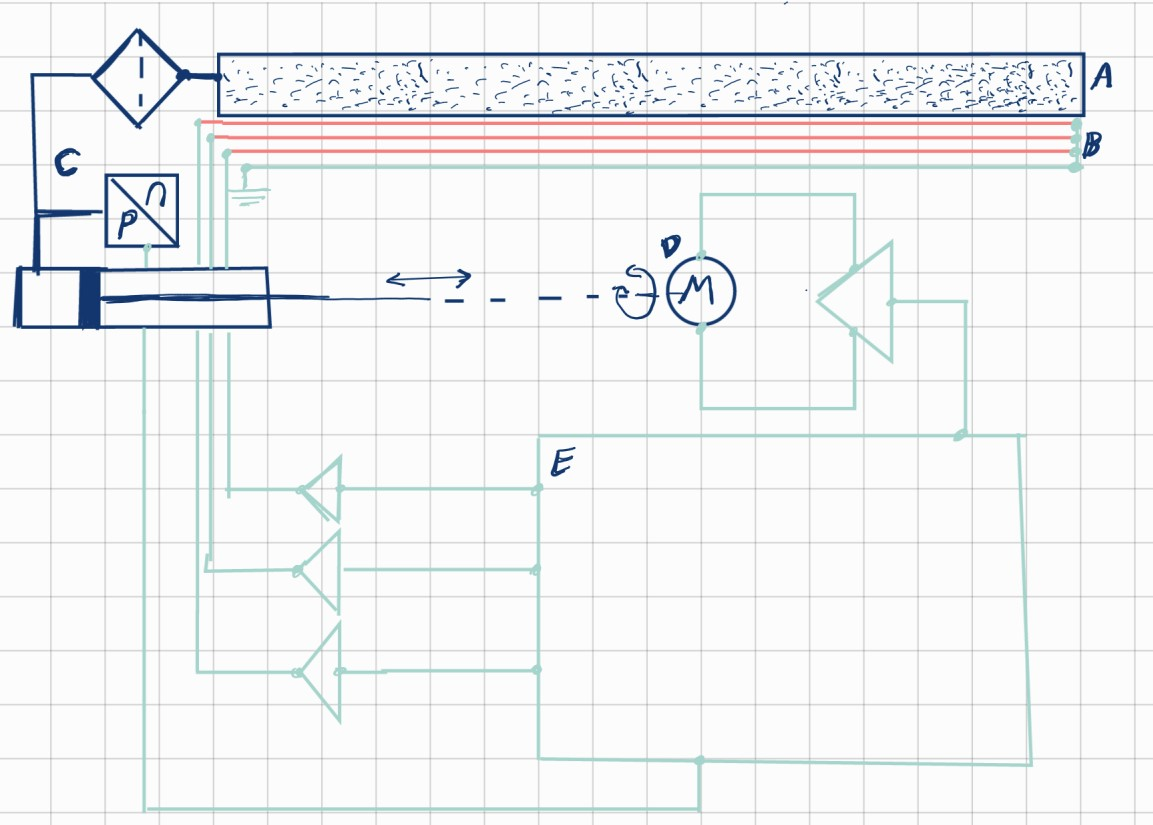
\includegraphics[width=\textwidth]{Schematic.jpg}
    \caption{Block diagram of the proposed device, with mechanical/pneumatic elements in blue, electronics in green,
    and SMA actuators in red. The particulate filled grasper (A) is attached to 3 SMA wires (B), and on one end to
    a filter, pressure sensor, and cylinder/syringe type pump (C). The pump is driven by a motor (D) and suitable
    gear assembly to achieve linear motion. The SMA wires and motor are all driven by the flight control unit (E).}
    \label{fig:schematic}
\end{figure}


To facilitate the jamming transition, a partial vacuum must be produced and maintained within the grasper.
The proposed design will use a servo driven syringe to draw a volume of air from the grasper,
activating the jamming behavior of the coffee grounds within. Two concepts for this mechanism are shown in Fig. {fig:pump}.
They are essentially the same, differing in the type of motor used.


\begin{figure}[H]
    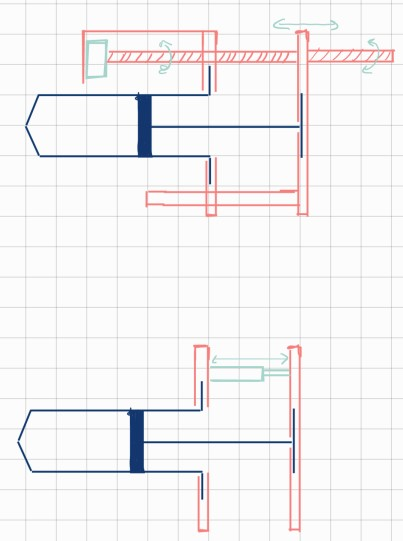
\includegraphics[width=\textwidth]{pump.jpg}
    \caption{Rough depiction of the proposed pump mechanism. Either a rotary motor and screw assembly (top) or
    a pre built linear actuator (bottom) will be used to extend or retract the syringes plunger. The mechanical assembly
    to link the motor and syringe (shown in red) will likely be 3D printed.}
    \label{fig:pump}
\end{figure}


The target pressure within the grasper with jamming activated will be 1/4 atm based on the procedure of Brown et al. \cite{brown_universal_2010}.
Assuming the following points, then  equation \ref{eqn:volume} gives the approximate volume of air to
remove from the grasper core to facilitate jamming.
\begin{itemize}
    \item 34\% porosity of the coffee grounds \cite{oliveros_experimental_2017}.
    \item The bulk of coffee grounds prevent significant volume reduction in
            the grasper core as a result of the pressure change.
    \item Pressure is equal within the grasper and the syringe.
    \item There is no leakage of air through any part of the syringe, grasper, or joining hardware.
\end{itemize}


\begin{eqn}[H]
    \begin{equation}
        \label{eqn:volume}
        V_b = (0.66 V_a) \frac{P_1 - P_2}{P_2}
    \end{equation}
    Where:
    \begin{itemize}
        \item $V_b$ is the volume draw out by the syringe.
        \item $V_a$ is the volume within the grasper, not accounting for the coffee grounds.
        \item $P_1$ is the normal pressure in the grasper, without jamming (1 atm).
        \item $P_2$ is the pressure in the grasper with jamming active (1/4 atm).
    \end{itemize}
\end{eqn}


The grasping device for this proof of concept is planned to be 50cm long. That will provide length to wrap at least on full turn around a perch
up to 15cm in diameter. The grasper core and SMA wires should be as small as possible, to minimize bulk and weight of the device.
Using 50mm of 3mm ID flex tubing for the grasper, $V_a$ is roughly $354 mm^3$.
That gives a volume $V_b$ of roughly $701 mm^3$. A 20mL syringe will provide sufficient volume, with room for error.


To maintain this vacuum, the driving servo must be capable of holding the 3/4 atm
% = 11.02196 psi = 0.075993739093 N / mm2
relative pressure the cylinder will be under. This force is given by equation \ref{eqn:force}.


\begin{eqn}[H]
    \begin{equation}
        \label{eqn:force}
        F = \pi (P_1 - P_2) (\frac{D}{2})^2
    \end{equation}
    Where:
    \begin{itemize}
        \item $F$ is the force sustained by the servo during jamming.
        \item $D$ is the inner diameter of the syringe.
        \item $P_1$ is the normal pressure in the grasper, without jamming (1 atm).
        \item $P_2$ is the pressure in the grasper with jamming active (1/4 atm).
    \end{itemize}
\end{eqn}


With a syringe having an inner diameter of 2cm, this gives a required force of 23.87 N or 5.37 lbs.
% 3/4 atm = 7.5994 N/cm2

\paragraph{Budget}


The estimated cost for components needed for this thesis is shown in table \ref{tab:grasper}. The design will utilize materials and tools available for student projects
in engineering facilities as much as possible, for example 3D printing or machining mechanical components, as well as other materials that are freely available, such as
coffee grounds and 20 mL syringes (which the author has left over from other projects).


The budget includes an estimated 7\% sales tax on all materials, as well as an additional 20\% of the total estimate
to account for any spare or replacement parts that are needed during development and testing.


\begin{table}[ht]
    \centering
    \caption{Estimated budget for the grasper design.}
    \label{tab:grasper}


    \begin{spreadtab}{{tabular}{|c|c|c|c||c|}}
        \hline
        @Item                       & @Supplier                                                                                                         & @Unit Cost (USD) & @Quantity & @Total Cost (USD) \\
        \hline
        @SMA Wire                   & @\href{https://www.kelloggsresearchlabs.com/product/round-wire/}{Kelloggs Research Labs}                          & 15.99 & 1 & [-1,0] * [-2,0] tag(start) \\
        @Kellogs Shipping           & @-                                                                                                                &  4.99 & 1 & [-1,0] * [-2,0] \\
        @Servo                      & @\href{https://www.digikey.com/en/products/detail/actuonix-motion-devices-inc/L16-50-150-6-R/11689514}{Digikey}   & 90.00 & 1 & [-1,0] * [-2,0] \\
        @Digikey Shipping           & @-                                                                                                                & 14.99 & 1 & [-1,0] * [-2,0] \\
        @Pneumatic Tube             & @\href{https://www.adafruit.com/product/4661}{Adafruit}                                                           &  2.50 & 1 & [-1,0] * [-2,0] \\
        @Amplifiers                 & @\href{https://www.adafruit.com/product/355}{Adafruit}                                                            &  2.25 & 3 & [-1,0] * [-2,0] \\
        @Arduino                    & @\href{https://www.adafruit.com/product/2378}{Adafruit}                                                           & 11.95 & 1 & [-1,0] * [-2,0] \\
        @FTDI Programmer            & @\href{https://www.adafruit.com/product/70}{Adafruit}                                                             & 19.95 & 1 & [-1,0] * [-2,0] \\
        @Pressure Sensor            & @\href{https://www.adafruit.com/product/3965}{Adafruit}                                                           & 29.95 & 1 & [-1,0] * [-2,0] \\
        @Limit Switches             & @\href{https://www.adafruit.com/product/818}{Adafruit}                                                            &  1.50 & 2 & [-1,0] * [-2,0] \\
        @Adafruit Shipping          & @-                                                                                                                &  5.08 & 1 & [-1,0] * [-2,0] \\
        @Syringe                    & @-                                                                                                                &     0 & 1 & [-1,0] * [-2,0] \\
        @Coffee Grounds             & @-                                                                                                                &     0 & 1 & [-1,0] * [-2,0] \\
        @PCB Material               & @\href{https://www.mcmaster.com/8521K873}{McMaster Carr}                                                          & 12.45 & 1 & [-1,0] * [-2,0] \\
        @McMaster Carr Shipping     & @-                                                                                                                & 10.02 & 1 & [-1,0] * [-2,0] \\
        @Mechanical Materials and Fabrication & @-                                                                                                      &     0 & 1 & [-1,0] * [-2,0] tag(pretax)\\
        @Tax                        & @- & sum(cell(start):cell(pretax)) * 0.07 & 1 & [-1,0] * [-2,0] tag(posttax) \\
        @Misc. Spares               & @- & sum(cell(start):cell(posttax)) * 0.2 & 1 & [-1,0] * [-2,0] tag(end) \\
        \hline
        \multicolumn{4}{|c||}{@Total} & sum(cell(start):cell(end)) \\
        \hline
    \end{spreadtab}
\end{table}


\paragraph{Evaluation}

Initial testing of this concept was done silicone tubing with inner diameter of 3mm and outer diameter of 5mm.
The tube was filled with coffee grounds. One end was plugged with a portion of a wooden skewer and secured with a zip tie,
and the other end secured with a zip tie to a 20mL syringe. 

Extending the syringe to its maximum volume (applying maximum vacuum) showed little change in the stiffness of the design.
This is possibly due to the thickness of the silicone tube. The actuator designed by Brown et al. \cite{brown_universal_2010} 
used a balloon, which is thinner and more flexible allowing the coffee grounds inside to bear the load of the vacuum. 
The tube in this test was thicker and stiffer, so less of the pressure was transferred to the coffee grounds inside,
preventing a change in stiffness. 

A second attempt with a thinner tube (a balloon, the long type used to make balloon animals) showed little improvement. 
There was no noticeable change in the stiffness of the device. This may indicate that the estimates for how much pressure is needed
or the volume of air withdrawn required to create this pressure are too low. Making the device capable of withdrawing more air would likely
result in too large and heavy of a final design. It is also possible that the failure of this concept is due to the small diameter of the
grasper not providing enough strength to resist deformation. Fixing this would also require the device to be larger and heavier.

